\documentclass{standalone}
\usepackage{tikz}
\usetikzlibrary{arrows,decorations.pathmorphing,decorations.shapes,backgrounds,fit,snakes,shapes,positioning}
\usepackage{times}
\usepackage[T1]{fontenc}
\renewcommand{\familydefault}{\sfdefault}
\begin{document}
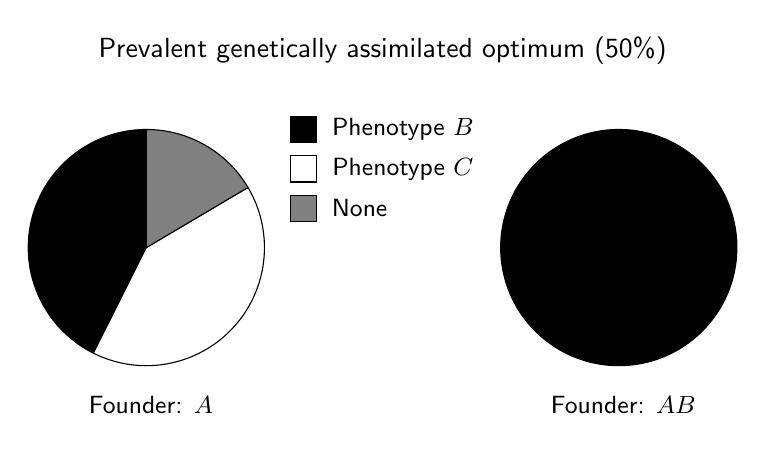
\begin{tikzpicture}[rectangle, minimum width=0.33cm, minimum height=0.333cm, bla/.style={draw, fill=white},neg/.style={draw, fill=black}, gri/.style={draw, fill=black!50}, gena/.style={font=\bf\fontsize{8.04}{9.67}\selectfont}, pac/.style={font=\fontsize{9}{7.035} \selectfont}]

\node at (5,5) {Prevalent genetically assimilated optimum (50\%)};
\filldraw[fill=black] (2, 2.5) -- +(90:1.5) arc (90:243.36:1.5) -- cycle;
\filldraw[fill=white] (2, 2.5) -- +(243.36:1.5) arc (243.36:390.6:1.5) -- cycle;
\filldraw[fill=black!50] (2, 2.5) -- +(390.6:1.5) arc (390.6:450:1.5) -- cycle;
\node[pac] at (2, 0.5) {Founder: $A$};
\node[neg] at (4, 4) {};
\node[pac] at (5.2, 4) {Phenotype $B$};
\node[bla] at (4, 3.5) {};
\node[pac] at (5.2, 3.5) {Phenotype $C$};
\node[gri] at (4, 3) {};
\node[pac] at (4.65, 3) {None};
\filldraw[fill=black] (8, 2.5) -- +(90:1.5) arc (90:450:1.5) -- cycle;
\filldraw[fill=white] (8, 2.5) -- +(450:1.5) arc (450:450:1.5) -- cycle;
\node[pac] at (8, 0.5) {Founder: $AB$};
\end{tikzpicture}
\end{document}
